\documentclass[12pt]{article}

% Настройка русского языка и шрифтов
\usepackage[utf8]{inputenc}
\usepackage[russian]{babel}
\usepackage[T2A]{fontenc}

% Математические пакеты
\usepackage{amsmath, amssymb, amsfonts}

% Настройка страницы
\usepackage{geometry}
\geometry{a4paper, margin=0.8in}

% Другие полезные пакеты
\usepackage{hyperref}
\usepackage{booktabs}
\usepackage{enumitem}
\usepackage{longtable}
\usepackage{graphicx}
\usepackage{xcolor}

% Определение стилей для комментариев
\definecolor{commentgray}{rgb}{0.4,0.4,0.4}
\definecolor{antigravityblue}{rgb}{0.0, 0.45, 0.74}

\newcommand{\commentary}[1]{{\small\itshape\color{commentgray} #1}}
\newcommand{\antigravity}[1]{{\small\color{antigravityblue}\textbf{Antigravity:} #1}}

% Настройка ссылок
\hypersetup{
    colorlinks=true,
    linkcolor=blue,
    filecolor=magenta,      
    urlcolor=cyan,
    pdftitle={Глубокий разбор: Градиентный бустинг (GBDT)},
}

\title{Глубокий разбор: Градиентный бустинг над решающими деревьями (GBDT)}
\author{Твой персональный гид по ML}
\date{\today}

\begin{document}

\subsection{Философское отличие: Бустинг vs Бэггинг}
Чтобы понять бустинг, нужно вспомнить случайный лес (бэггинг). 
\begin{itemize}
    \item \textbf{Бэггинг} (Random Forest) строит много глубоких, умных деревьев \textbf{независимо} и усредняет их. Это борется с \textbf{разбросом} (variance).
    \item \textbf{Бустинг} строит цепочку из очень простых («глупых») деревьев \textbf{последовательно}. Каждое следующее дерево исправляет ошибки всех предыдущих. Это борется со \textbf{смещением} (bias).
\end{itemize}

\commentary{Бустинг можно представить как гольфиста, цель которого — загнать мяч в лунку. Здесь положение мяча — ответ композиции. Каждый следующий удар — это та поправка, которую вносит очередной базовый алгоритм. Если гольфист всё делает правильно, то функция потерь будет уменьшаться с каждым ударом.}

\begin{figure}[h]
    \centering
    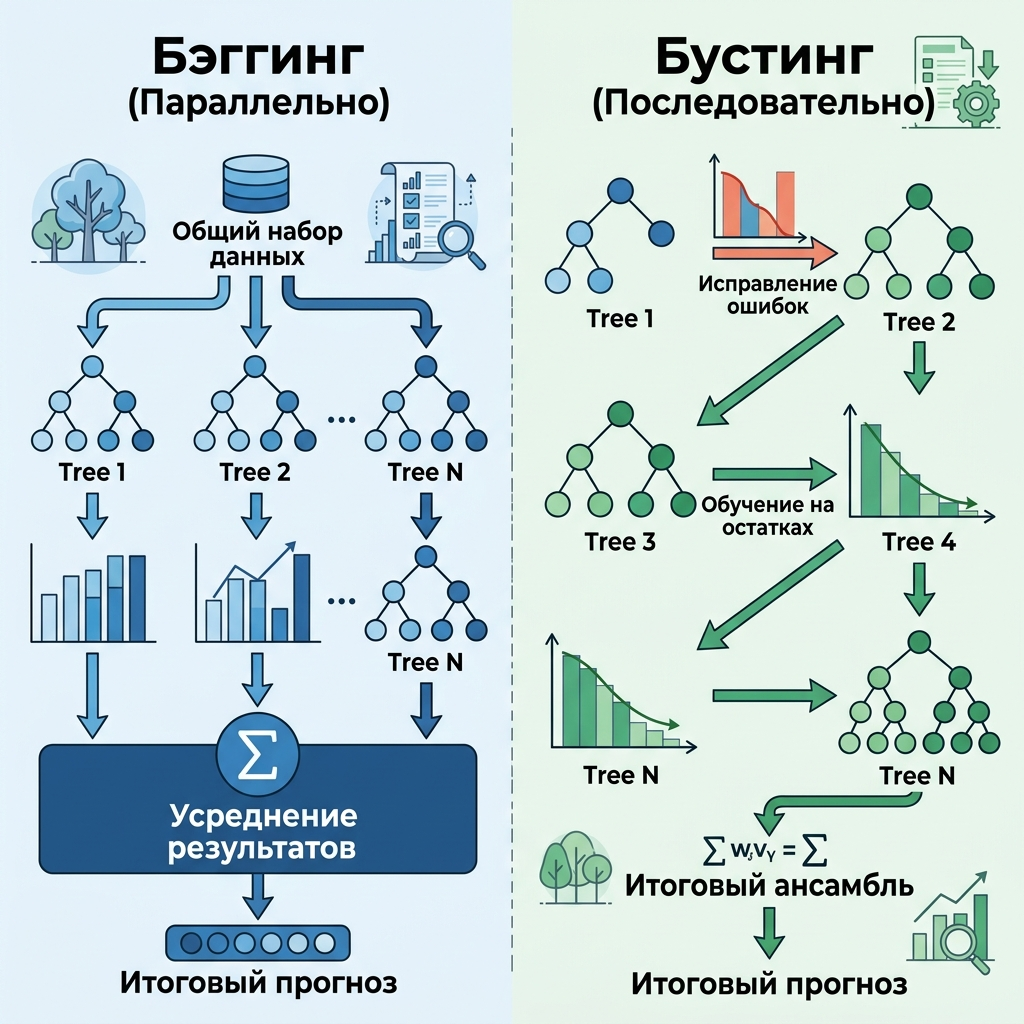
\includegraphics[width=0.7\textwidth]{boosting_bagging.png}
    \caption{Концептуальное различие между Бустингом и Бэггингом.}
\end{figure}

\subsection{Математика: Градиентный спуск в функциональном пространстве}
В градиентном бустинге мы меняем \textbf{саму функцию} $a(x)$.

Представь, что текущая композиция $a_{k-1}$ выдает предсказания. Мы хотим добавить к ней дерево $b_k$, чтобы общая ошибка упала. 
\begin{enumerate}
    \item \textbf{Градиент}: $g_i = \frac{\partial \mathcal{L}(y_i, z)}{\partial z} \Big|_{z = a_{k-1}(x_i)}$. Это число говорит, куда нужно «подвинуть» предсказание для уменьшения ошибки.
    \item \textbf{Антиградиент}: Для наискорейшего уменьшения функции потерь нам необходимо шагнуть в сторону её антиградиента по вектору предсказаний текущей композиции, то есть в сторону вектора $-g$.
    \item \textbf{Универсальность}: Для каждого объекта очередной алгоритм $b_k$ в бустинге обучается предсказывать антиградиент функции потерь по предсказанию модели. Это наблюдение позволяет обобщить подход построения бустинга на \textbf{произвольную дифференцируемую функцию потерь}.
\end{enumerate}

\begin{figure}[h]
    \centering
    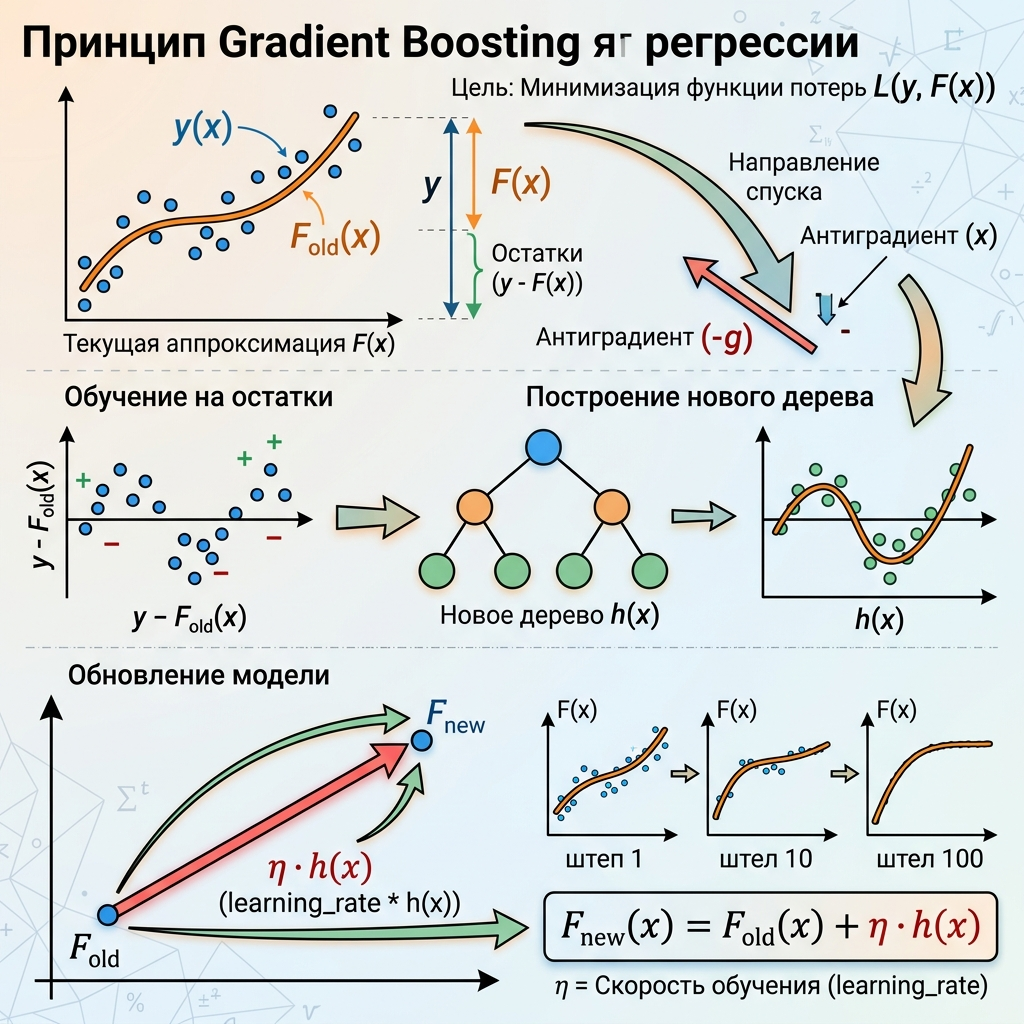
\includegraphics[width=0.6\textwidth]{gbdt_math.png}
    \caption{Процесс обучения нового дерева на антиградиент функции потерь.}
\end{figure}

\subsection{Секрет успеха: Почему деревья неглубокие?}
В GBDT базовые деревья обычно имеют глубину всего \textbf{3–6 уровней}. 
Смысл бустинга в том, чтобы каждое дерево вносило \textbf{крошечный, но точный вклад}. Тысяча маленьких уточнений работают лучше, чем пять больших и грубых.

\subsection{Борьба с «жадностью»: Регуляризация}
\begin{itemize}
    \item \textbf{Learning Rate (Shrinkage)}: Мы берем лишь малую часть предсказаний нового дерева (например, 0.1). Это делает алгоритм устойчивым к шуму.
    \item \textbf{Стохастичность}: Использование случайных подмножеств данных для построения каждого дерева (Stochastic Gradient Boosting).
\end{itemize}

\subsection{Тройка лидеров: XGBoost, LightGBM, CatBoost}

\begin{figure}[h]
    \centering
    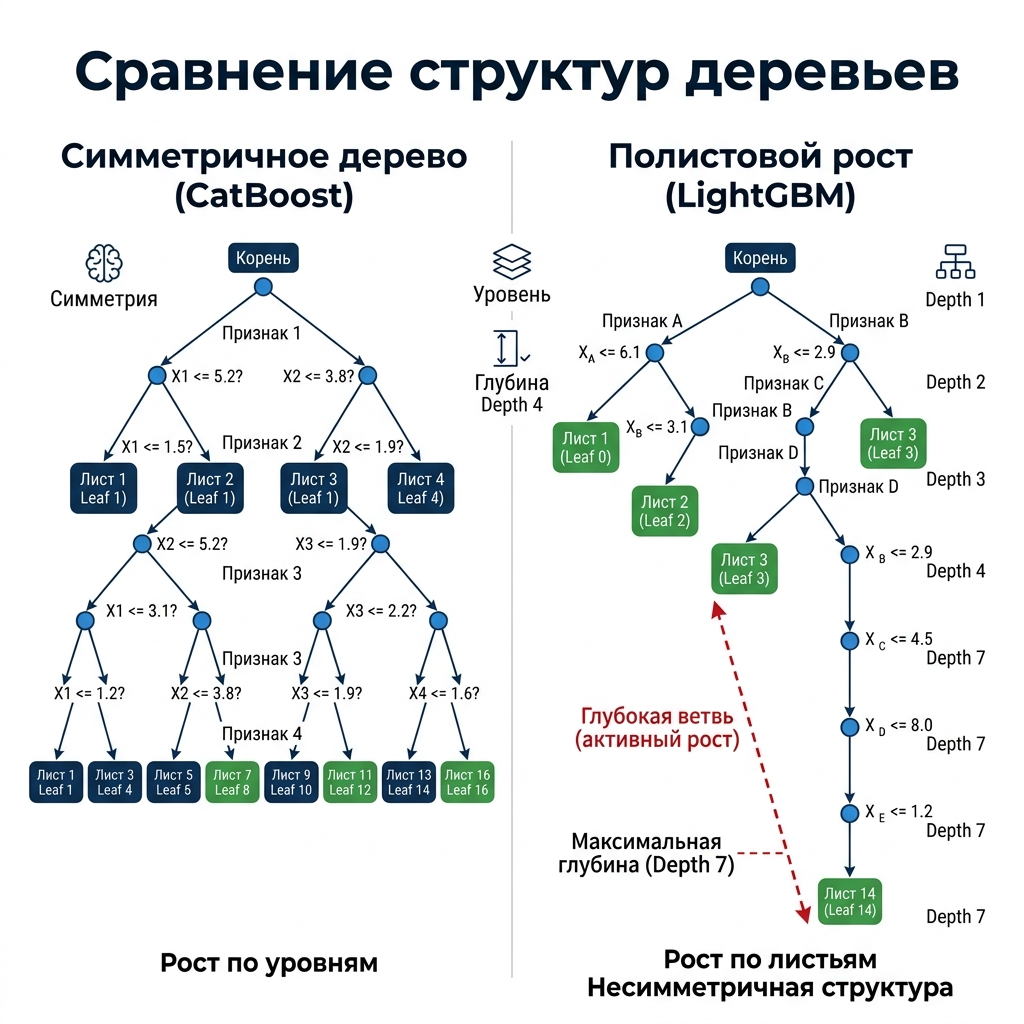
\includegraphics[width=0.7\textwidth]{tree_growth.png}
    \caption{Различия в структуре деревьев: CatBoost (симметричные) vs LightGBM (полистовые).}
\end{figure}

\subsection{CatBoost (от Яндекса)}
\begin{itemize}
    \item \textbf{Симметричные деревья}: Все узлы на одном уровне используют один и тот же признак.
    \item \textbf{Категориальные признаки}: Продвинутые схемы кодирования "из коробки".
\end{itemize}

\subsection{LightGBM (от Microsoft)}
\begin{itemize}
    \item \textbf{Leaf-wise рост}: Выбирает самый «перспективный» лист и разбивает его.
    \item \textbf{Гистограммный метод}: Сжатие признаков в «корзины» для ускорения.
\end{itemize}

\subsection{XGBoost}
\begin{itemize}
    \item \textbf{Вторая производная}: Использует разложение Тейлора до второго порядка (Гессиан) для точности.
\end{itemize}

\subsection{Интерпретация: Feature Importance}
\begin{enumerate}
    \item \textbf{Weight (Frequency)}: Частота использования признака.
    \item \textbf{Gain}: Суммарное падение ошибки от признака.
    \item \textbf{Permutation Importance}: Падение качества при перемешивании значений.
\end{enumerate}

\vspace{1cm}
\commentary{Главное при работе с бустингом — следить за графиком лосса на валидации. Как только ошибка на валидации перестала падать, а на трейне продолжает — немедленно останавливайся (это называется Early Stopping).}

\antigravity{Для большинства табличных задач CatBoost — это выбор по умолчанию благодаря отличной работе с категориями и регуляризации.}

\end{document}
